\section{Exercise D.}
Two processes P and Q are connected in a ring using two channels, and they constantly rotate a message m. At any one time, there is only one copy of m in the system. Each process’s state consists of the number of times it has received m, and P sends m first. At a certain point, P has the message and its state is 101. Immediately after sending m, P initiates the snapshot algorithm. Explain the operation of the algorithm in this case, giving the possible global state(s) reported by it.\\\\
The snapshot algorithm as described in \emph{Distributed Systems — Concepts \& Design} p. 616\\

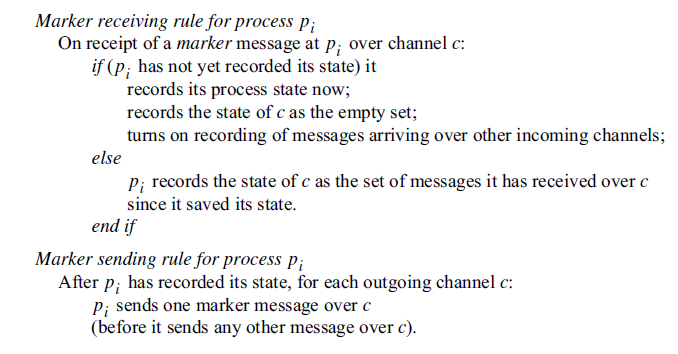
\includegraphics[scale=0.7]{Snapshot-Algorithm}\\

Since P initiates the algorithm we look at the ‘Marker sending rule for process’ first, therefore P records its state to begin with, and since it has received the message M 101 times, this value will be stored. P only has one channel and therefore it sends a marker message along it to Q, and afterwards turns on recording of messages arriving over other incoming channels.

Q at this time receives M and therefore raises its state to 102 and sends the message on again. Shortly after Q receives the Marker message from P and therefore starts the “Marker receiving rule for process”. Since it has not yet recorded its state it does so, and then records the incoming channel as empty. No other incoming channels exists so the algorithm is done.

\newpage